\section{ADDITIONAL EXPERIMENTS}







\subsection{Main results}

\begin{figure*}[htb]
    \centering
    \begin{subfigure}[b]{0.475\textwidth}
        \centering
        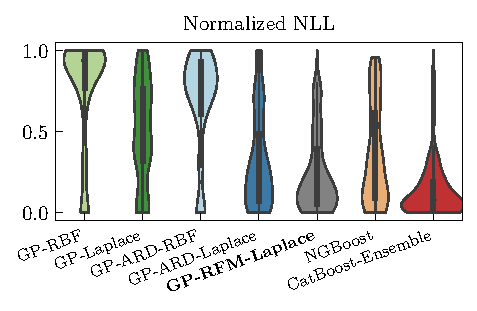
\includegraphics[trim=0 40 0 0, clip, width=\textwidth]{figures/tabularbenchmark_nll.pdf}
    \end{subfigure}
    \hfill
    \begin{subfigure}[b]{0.475\textwidth}  
        \centering 
        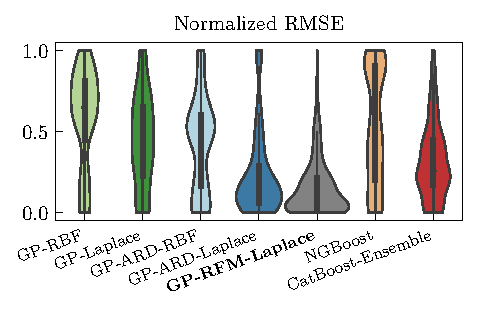
\includegraphics[trim=0 40 0 0, clip, width=\textwidth]{figures/tabularbenchmark_rmse.pdf}
    \end{subfigure}
    % \vskip\baselineskip
    \begin{subfigure}[b]{0.475\textwidth}   
        \centering 
        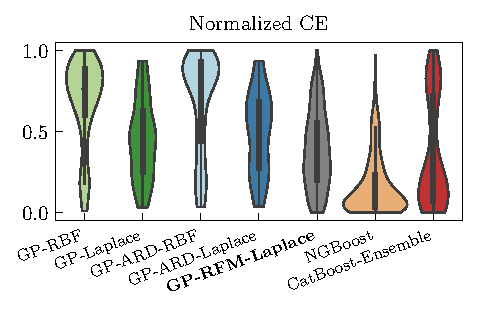
\includegraphics[width=\textwidth]{figures/tabularbenchmark_coverage.pdf}
    \end{subfigure}
    \hfill
    \begin{subfigure}[b]{0.475\textwidth}   
        \centering 
        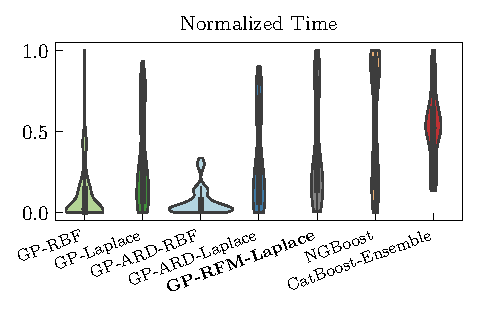
\includegraphics[width=\textwidth]{figures/tabularbenchmark_time.pdf}
    \end{subfigure}
    \caption{
        \hl{title TODO} results on tabular benchmark datasets
        \daniel{explanation: Every dataset of the 16 tabular benchmark dataset; tabular benchmark has more datasets/features/samples than uci benchmark we use; all hyperparameters are tuned; run everything for 20 seeds; for each dataset and metric we normalize the results of all methods in $[0,1]$; violin plot.}
        \daniel{use word 'coverage error'}
        } 
    \label{fig:main-tabular-benchmark-app}
\end{figure*}

\begin{figure*}[htb]
    \centering
    \begin{subfigure}[b]{0.475\textwidth}
        \centering
        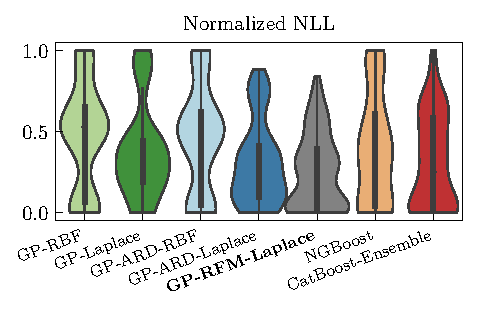
\includegraphics[trim=0 40 0 0, clip, width=\textwidth]{figures/uci_nll.pdf}
    \end{subfigure}
    \hfill
    \begin{subfigure}[b]{0.475\textwidth}  
        \centering 
        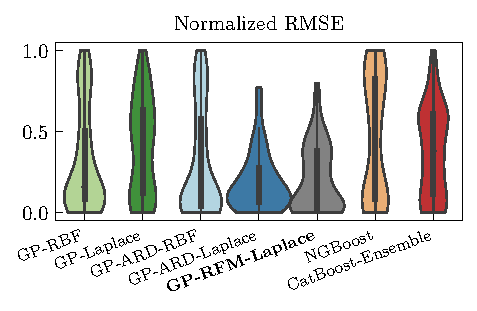
\includegraphics[trim=0 40 0 0, clip, width=\textwidth]{figures/uci_rmse.pdf}
    \end{subfigure}
    % \vskip\baselineskip
    \begin{subfigure}[b]{0.475\textwidth}   
        \centering 
        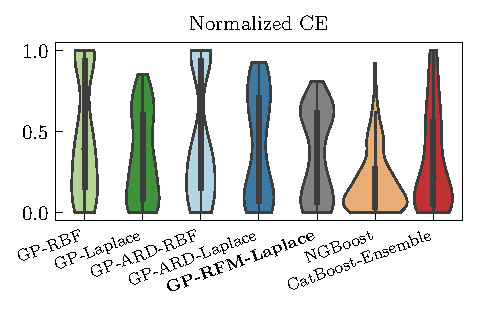
\includegraphics[width=\textwidth]{figures/uci_coverage.pdf}
    \end{subfigure}
    \hfill
    \begin{subfigure}[b]{0.475\textwidth}   
        \centering 
        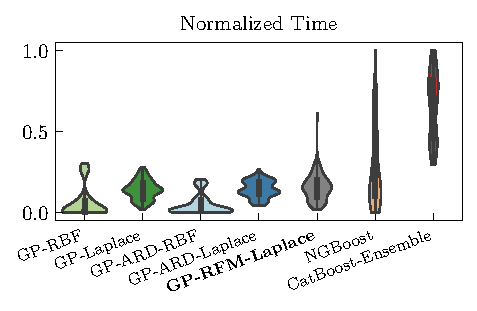
\includegraphics[width=\textwidth]{figures/uci_time.pdf}
    \end{subfigure}
    \caption{
        \hl{title TODO} results on UCI datasets. Complementary to \Cref{fig:main-tabular-benchmark}.
        \daniel{explanation: same as in \Cref{fig:main-tabular-benchmark}}
        } 
    \label{fig:main-uci}
\end{figure*}



\subsection{Comparative feature evaluation}



\begin{figure*}[htb]
    \centering
    \begin{subfigure}[b]{0.475\textwidth}
        \centering
        % \includegraphics{figuresTikz/feature_importance_nll}
        % \tikzsetnextfilename{feature_importance_nll}
        \begin{tikzpicture}[baseline]

\pgfplotstableread[col sep=comma]{./data/feature_importance_metrics.csv}{\datatable};
\begin{axis}[
width=\columnwidth,
height=.7\columnwidth,
ylabel={NLL},
xlabel={Fraction of remaining features},
title={Performance when removing features},
% ymax=0.3,
legend style={font=\tiny, 
	fill opacity=0.6, text opacity =1,
        at={(0.02, 0.02)},anchor=south west,
        row sep=-3pt,
        },
legend cell align={left},
% ytick={0, 0.08}, % Define the desired y tick positions
xtick={60, 70, 80, 90, 100}, % Define the desired y tick positions
xticklabels={60\%, 70\%, 80\%, 90\%, 100\%},
yticklabel style={
	% /pgf/number format/fixed, % Use fixed point notation
	% /pgf/number format/precision=2, % Set the number of decimal places
	% /pgf/number format/fixed zerofill, % Fill in trailing zeros
        },
% ymode=log,
]

% GP-RBF
\addplot+ [lightgreen, mark=*, 
mark options={solid},
thick,
% error bars/.cd,
% x dir=both,x explicit,
% y dir=both,y explicit,
% error bar style={solid}
]
table[x=features,y=GP_RBF_NLPD_mean,y error=GP_RBF_NLPD_std] {\datatable};


% GP-Laplace
\addplot+ [darkgreen, mark=*, 
mark options={solid},
thick,
% error bars/.cd,
% x dir=both,x explicit,
% y dir=both,y explicit,
% error bar style={solid}
]
table[x=features,y=GP_Laplace_NLPD_mean,y error=GP_Laplace_NLPD_std] {\datatable};


% GP-ARD-RBF
\addplot+ [lightblue, mark=*, 
mark options={solid},
thick,
dotted,
% error bars/.cd,
% x dir=both,x explicit,
% y dir=both,y explicit,
% error bar style={solid}
]
table[x=features,y=GP_ARD_RBF_NLPD_mean,y error=GP_ARD_RBF_NLPD_std] {\datatable};


% GP-ARD-Laplace
\addplot+ [darkblue, mark=*, 
mark options={solid},
thick,
dotted,
% error bars/.cd,
% x dir=both,x explicit,
% y dir=both,y explicit,
% error bar style={solid}
]
table[x=features,y=GP_ARD_Laplace_NLPD_mean,y error=GP_ARD_Laplace_NLPD_std] {\datatable};


% RFM
\addplot+ [black, mark=*, 
mark options={solid},
thick,
% error bars/.cd,
% x dir=both,x explicit,
% y dir=both,y explicit,
% error bar style={solid}
]
table[x=features,y=GP_RFM_Laplace_NLPD_mean,y error=GP_RFM_Laplace_NLPD_std] {\datatable};


% NG-Boost
\addplot+ [orange, mark=*, 
mark options={solid},
thick,
dashed,
% error bars/.cd,
% x dir=both,x explicit,
% y dir=both,y explicit,
% error bar style={solid}
]
table[x=features,y=NG_Boost_NLPD_mean,y error=GP_RFM_Laplace_NLPD_std] {\datatable};


% Cat-Boost-Ensemble
\addplot+ [red, mark=*, 
mark options={solid},
thick,
dashed,
% error bars/.cd,
% x dir=both,x explicit,
% y dir=both,y explicit,
% error bar style={solid}
]
table[x=features,y=Cat_Boost_Ensemble_NLPD_mean,y error=Cat_Boost_Ensemble_NLPD_std] {\datatable};



\legend{
    {GP-RBF},
    {GP-Laplace},
    {GP-ARD-RBF},
    {GP-ARD-Laplace},
    {GP-RFM-Laplace}, 
    {NGBoost},
    {CatBoost-Ensemble}
}

\end{axis}
\end{tikzpicture}
    \end{subfigure}
    \hfill
    \begin{subfigure}[b]{0.475\textwidth}  
        \centering
        % \includegraphics{figuresTikz/feature_importance_rmse}
        % \tikzsetnextfilename{feature_importance_rmse}
        \begin{tikzpicture}[baseline]

\pgfplotstableread[col sep=comma]{./data/feature_importance_metrics.csv}{\datatable};
\begin{axis}[
width=1\columnwidth,
height=.7\columnwidth,
ylabel={RMSE},
xlabel={Fraction of remaining features},
title={Performance when removing features},
% ymax=0.3,
legend style={font=\tiny, 
	fill opacity=0.6, text opacity =1,
        at={(0.02, 0.02)},anchor=south west,
        row sep=-3pt,
        },
legend cell align={left},
% ytick={0, 0.08}, % Define the desired y tick positions
xtick={60, 70, 80, 90, 100}, % Define the desired y tick positions
xticklabels={60\%, 70\%, 80\%, 90\%, 100\%},
yticklabel style={
	% /pgf/number format/fixed, % Use fixed point notation
	% /pgf/number format/precision=2, % Set the number of decimal places
	% /pgf/number format/fixed zerofill, % Fill in trailing zeros
        },
% ymode=log,
]

% GP-RBF
\addplot+ [lightgreen, mark=*, 
mark options={solid},
thick,
% error bars/.cd,
% x dir=both,x explicit,
% y dir=both,y explicit,
% error bar style={solid}
]
table[x=features,y=GP_RBF_RMSE_mean,y error=GP_RBF_RMSE_std] {\datatable};


% GP-Laplace
\addplot+ [darkgreen, mark=*, 
mark options={solid},
thick,
% error bars/.cd,
% x dir=both,x explicit,
% y dir=both,y explicit,
% error bar style={solid}
]
table[x=features,y=GP_Laplace_RMSE_mean,y error=GP_Laplace_RMSE_std] {\datatable};


% GP-ARD-RBF
\addplot+ [lightblue, mark=*, 
mark options={solid},
thick,
dotted,
% error bars/.cd,
% x dir=both,x explicit,
% y dir=both,y explicit,
% error bar style={solid}
]
table[x=features,y=GP_ARD_RBF_RMSE_mean,y error=GP_ARD_RBF_RMSE_std] {\datatable};


% GP-ARD-Laplace
\addplot+ [darkblue, mark=*, 
mark options={solid},
thick,
dotted,
% error bars/.cd,
% x dir=both,x explicit,
% y dir=both,y explicit,
% error bar style={solid}
]
table[x=features,y=GP_ARD_Laplace_RMSE_mean,y error=GP_ARD_Laplace_RMSE_std] {\datatable};


% RFM
\addplot+ [black, mark=*, 
mark options={solid},
thick,
% error bars/.cd,
% x dir=both,x explicit,
% y dir=both,y explicit,
% error bar style={solid}
]
table[x=features,y=GP_RFM_Laplace_RMSE_mean,y error=GP_RFM_Laplace_RMSE_std] {\datatable};


% NG-Boost
\addplot+ [orange, mark=*, 
mark options={solid},
thick,
dashed,
% error bars/.cd,
% x dir=both,x explicit,
% y dir=both,y explicit,
% error bar style={solid}
]
table[x=features,y=NG_Boost_RMSE_mean,y error=GP_RFM_Laplace_RMSE_std] {\datatable};


% Cat-Boost-Ensemble
\addplot+ [red, mark=*, 
mark options={solid},
thick,
dashed,
% error bars/.cd,
% x dir=both,x explicit,
% y dir=both,y explicit,
% error bar style={solid}
]
table[x=features,y=Cat_Boost_Ensemble_RMSE_mean,y error=Cat_Boost_Ensemble_RMSE_std] {\datatable};



\legend{
    {GP-RBF},
    {GP-Laplace},
    {GP-ARD-RBF},
    {GP-ARD-Laplace},
    {GP-RFM-Laplace}, 
    {NGBoost},
    {CatBoost Ensemble}
}

\end{axis}
\end{tikzpicture}
    \end{subfigure}
    \caption{NLL (left) and RMSE (right) when removing the most important features according to the diagonal of the RFM weight matrix.} 
    \label{fig:feature-importance}
\end{figure*}
    







\subsection{Toy data set}

\begin{figure}[htb]
    \centering
    % \includegraphics{figuresTikz/toy_data_rmse}
    % \tikzsetnextfilename{toy_data_rmse}
    \begin{tikzpicture}[baseline]

\pgfplotstableread[col sep=comma]{./data/toy_data_metrics.csv}{\datatable};
\begin{axis}[
width=0.5\columnwidth,
height=.35\columnwidth,
ylabel={RMSE},
xlabel={features},
title={Toy data with feature correlation},
xmin=19,
xmax=131,
% ymin=0,
% ymax=0.33,
legend style={font=\tiny, 
	fill opacity=0.6, text opacity =1,
        % at={(1.,1)},anchor=north east,
        row sep=-3pt,
        },
legend cell align={left},
% ytick={0, 0.08}, % Define the desired y tick positions
xtick={10, 30, 50, 70, 90, 110, 130}, % Define the desired y tick positions
yticklabel style={
	% /pgf/number format/fixed, % Use fixed point notation
	% /pgf/number format/precision=2, % Set the number of decimal places
	% /pgf/number format/fixed zerofill, % Fill in trailing zeros
        },
% ymode=log,
]


% RFM full
\addplot+ [black, 
mark=*, 
mark options={solid},
% mark size=5pt, 
thick,
error bars/.cd,
x dir=both,x explicit,
y dir=both,y explicit,
error bar style={solid}
]
table[x=features,y=GP_RFM_Laplace_full_RMSE_mean,y error=GP_RFM_Laplace_full_RMSE_std] {\datatable};

% % RFM diag
% \addplot+ [red, mark=x, mark size=5pt, thick,
% error bars/.cd,
% x dir=both,x explicit,
% y dir=both,y explicit,
% error bar style={solid}
% ]
% table[x=features,y=GP_RFM_Laplace_diag_RMSE_mean,y error=GP_RFM_Laplace_diag_RMSE_std] {\datatable};

% Laplace
\addplot+ [darkgreen, 
mark=*, 
mark options={solid},
% mark size=5pt, 
thick,
error bars/.cd,
x dir=both,x explicit,
y dir=both,y explicit,
error bar style={solid}
]
table[x=features,y=GP_Laplace_RMSE_mean,y error=GP_Laplace_RMSE_std] {\datatable};

% ARD-Laplace
\addplot+ [darkblue, 
dotted,
mark=*, 
mark options={solid},
% mark size=5pt, 
thick,
error bars/.cd,
x dir=both,x explicit,
y dir=both,y explicit,
error bar style={solid}
]
table[x=features,y=GP_ARD_Laplace_RMSE_mean,y error=GP_ARD_Laplace_RMSE_std] {\datatable};

% NG-boost
\addplot+ [orange, 
dashed,
mark=*, 
mark options={solid},
% mark size=5pt, 
thick,
error bars/.cd,
x dir=both,x explicit,
y dir=both,y explicit,
error bar style={solid}
]
table[x=features,y=NG_Boost_RMSE_mean,y error=NG_Boost_RMSE_std] {\datatable};

% Cat-Boost Ensemble
\addplot+ [red, 
dashed,
mark=*, 
mark options={solid},
% mark size=5pt, 
thick,
error bars/.cd,
x dir=both,x explicit,
y dir=both,y explicit,
error bar style={solid}
]
table[x=features,y=Cat_Boost_Ensemble_RMSE_mean,y error=Cat_Boost_Ensemble_RMSE_std] {\datatable};



\legend{
    {GP-RFM}, 
    {GP-Laplace},
    % {GP-RFM-diag},
    {GP-ARD-Laplace},
    {NGBoost},
    {CatBoost Ensemble}
}

\end{axis}
\end{tikzpicture}
    \caption{
        \hl{Title TODO} Complementary to \Cref{fig:toy-data-nll} but showing RMSE instead of NLL here.
        \daniel{Explanation: Same as in \Cref{fig:toy-data-nll}.}
        }
    \label{fig:toy-data-rmse}
\end{figure}

\hl{Include figure about learnt feature matrix in RFM, RFM-diag and ARD-Laplace as comprison}








\subsection{Distribution shift}


\begin{figure*}[htb]
    \centering
    \begin{subfigure}[b]{0.475\textwidth}
        \centering
        % \includegraphics{figuresTikz/ood_covariate_nll}
        % \tikzsetnextfilename{ood_covariate_nll}
        \begin{tikzpicture}[baseline]

\pgfplotstableread[col sep=comma]{./data/ood_covariate_metrics.csv}{\datatable};
\begin{axis}[
width=\columnwidth,
height=.7\columnwidth,
% ylabel={NLL},
% xlabel={},
title={NLL},
ymax=2,
legend style={font=\tiny, 
	fill opacity=0.6, text opacity =1,
        at={(0.02, 0.98)},anchor=north west,
        row sep=-3pt,
        },
legend cell align={left},
% ytick={0, 0.08}, % Define the desired y tick positions
xtick={0, 1,2,3,4}, % Define the desired y tick positions
xticklabels={ID, OOD-1, OOD-2, OOD-3, OOD-4},
yticklabel style={
	% /pgf/number format/fixed, % Use fixed point notation
	% /pgf/number format/precision=2, % Set the number of decimal places
	% /pgf/number format/fixed zerofill, % Fill in trailing zeros
        },
% ymode=log,
]

% GP-RBF
\addplot+ [lightgreen, mark=*, 
mark options={solid},
thick,
% error bars/.cd,
% x dir=both,x explicit,
% y dir=both,y explicit,
% error bar style={solid}
]
table[x=test_level,y=GP_RBF_NLPD_mean,y error=GP_RBF_NLPD_std] {\datatable};


% GP-Laplace
\addplot+ [darkgreen, mark=*, 
mark options={solid},
thick,
% error bars/.cd,
% x dir=both,x explicit,
% y dir=both,y explicit,
% error bar style={solid}
]
table[x=test_level,y=GP_Laplace_NLPD_mean,y error=GP_Laplace_NLPD_std] {\datatable};


% GP-ARD-RBF
\addplot+ [lightblue, mark=*, 
mark options={solid},
thick,
dotted,
% error bars/.cd,
% x dir=both,x explicit,
% y dir=both,y explicit,
% error bar style={solid}
]
table[x=test_level,y=GP_ARD_RBF_NLPD_mean,y error=GP_ARD_RBF_NLPD_std] {\datatable};


% GP-ARD-Laplace
\addplot+ [darkblue, mark=*, 
mark options={solid},
thick,
dotted,
% error bars/.cd,
% x dir=both,x explicit,
% y dir=both,y explicit,
% error bar style={solid}
]
table[x=test_level,y=GP_ARD_Laplace_NLPD_mean,y error=GP_ARD_Laplace_NLPD_std] {\datatable};


% RFM
\addplot+ [black, mark=*, 
mark options={solid},
thick,
% error bars/.cd,
% x dir=both,x explicit,
% y dir=both,y explicit,
% error bar style={solid}
]
table[x=test_level,y=GP_RFM_Laplace_NLPD_mean,y error=GP_RFM_Laplace_NLPD_std] {\datatable};


% NG-Boost
\addplot+ [orange, mark=*, 
mark options={solid},
thick,
dashed,
% error bars/.cd,
% x dir=both,x explicit,
% y dir=both,y explicit,
% error bar style={solid}
]
table[x=test_level,y=NG_Boost_NLPD_mean,y error=GP_RFM_Laplace_NLPD_std] {\datatable};


% Cat-Boost-Ensemble
\addplot+ [red, mark=*, 
mark options={solid},
thick,
dashed,
% error bars/.cd,
% x dir=both,x explicit,
% y dir=both,y explicit,
% error bar style={solid}
]
table[x=test_level,y=Cat_Boost_Ensemble_NLPD_mean,y error=Cat_Boost_Ensemble_NLPD_std] {\datatable};



% \legend{
%     {GP-RBF},
%     {GP-Laplace},
%     {GP-ARD-RBF},
%     {GP-ARD-Laplace},
%     {GP-RFM-Laplace}, 
%     {NGBoost},
%     {CatBoost-Ensemble}
% }

\end{axis}
\end{tikzpicture}
    \end{subfigure}
    \hfill
    \begin{subfigure}[b]{0.475\textwidth}  
        \centering
        % \includegraphics{figuresTikz/ood_covariate_rmse}
        % \tikzsetnextfilename{ood_covariate_rmse}
        \begin{tikzpicture}[baseline]

\pgfplotstableread[col sep=comma]{./data/ood_covariate_metrics.csv}{\datatable};
\begin{axis}[
width=\columnwidth,
height=.7\columnwidth,
% ylabel={RMSE},
% xlabel={},
title={RMSE},
% ymax=2,
legend style={font=\tiny, 
	fill opacity=0.6, text opacity =1,
        at={(0.02, 0.98)},anchor=north west,
        row sep=-3pt,
        },
legend cell align={left},
% ytick={0, 0.08}, % Define the desired y tick positions
xtick={0, 1,2,3,4}, % Define the desired y tick positions
xticklabels={ID, OOD-1, OOD-2, OOD-3, OOD-4},
yticklabel style={
	% /pgf/number format/fixed, % Use fixed point notation
	% /pgf/number format/precision=2, % Set the number of decimal places
	% /pgf/number format/fixed zerofill, % Fill in trailing zeros
        },
% ymode=log,
]

% GP-RBF
\addplot+ [lightgreen, mark=*, 
mark options={solid},
thick,
% error bars/.cd,
% x dir=both,x explicit,
% y dir=both,y explicit,
% error bar style={solid}
]
table[x=test_level,y=GP_RBF_RMSE_mean,y error=GP_RBF_RMSE_std] {\datatable};


% GP-Laplace
\addplot+ [darkgreen, mark=*, 
mark options={solid},
thick,
% error bars/.cd,
% x dir=both,x explicit,
% y dir=both,y explicit,
% error bar style={solid}
]
table[x=test_level,y=GP_Laplace_RMSE_mean,y error=GP_Laplace_RMSE_std] {\datatable};


% GP-ARD-RBF
\addplot+ [lightblue, mark=*, 
mark options={solid},
thick,
dotted,
% error bars/.cd,
% x dir=both,x explicit,
% y dir=both,y explicit,
% error bar style={solid}
]
table[x=test_level,y=GP_ARD_RBF_RMSE_mean,y error=GP_ARD_RBF_RMSE_std] {\datatable};


% GP-ARD-Laplace
\addplot+ [darkblue, mark=*, 
mark options={solid},
thick,
dotted,
% error bars/.cd,
% x dir=both,x explicit,
% y dir=both,y explicit,
% error bar style={solid}
]
table[x=test_level,y=GP_ARD_Laplace_RMSE_mean,y error=GP_ARD_Laplace_RMSE_std] {\datatable};


% RFM
\addplot+ [black, mark=*, 
mark options={solid},
thick,
% error bars/.cd,
% x dir=both,x explicit,
% y dir=both,y explicit,
% error bar style={solid}
]
table[x=test_level,y=GP_RFM_Laplace_RMSE_mean,y error=GP_RFM_Laplace_RMSE_std] {\datatable};


% NG-Boost
\addplot+ [orange, mark=*, 
mark options={solid},
thick,
dashed,
% error bars/.cd,
% x dir=both,x explicit,
% y dir=both,y explicit,
% error bar style={solid}
]
table[x=test_level,y=NG_Boost_RMSE_mean,y error=GP_RFM_Laplace_RMSE_std] {\datatable};


% Cat-Boost-Ensemble
\addplot+ [red, mark=*, 
mark options={solid},
thick,
dashed,
% error bars/.cd,
% x dir=both,x explicit,
% y dir=both,y explicit,
% error bar style={solid}
]
table[x=test_level,y=Cat_Boost_Ensemble_RMSE_mean,y error=Cat_Boost_Ensemble_RMSE_std] {\datatable};



\legend{
    {GP-RBF},
    {GP-Laplace},
    {GP-ARD-RBF},
    {GP-ARD-Laplace},
    {GP-RFM-Laplace}, 
    {NGBoost},
    {CatBoost-Ensemble}
}

\end{axis}
\end{tikzpicture}
    \end{subfigure}
    % \vskip\baselineskip
    \begin{subfigure}[b]{0.475\textwidth}   
        \centering
        % \includegraphics{figuresTikz/ood_covariate_coverage}
        % \tikzsetnextfilename{ood_covariate_coverage}
        \begin{tikzpicture}[baseline]

\pgfplotstableread[col sep=comma]{./data/ood_covariate_metrics.csv}{\datatable};
\begin{axis}[
width=\columnwidth,
height=.7\columnwidth,
% ylabel={Coverage},
% xlabel={},
title={Coverage Error},
% ymax=2,
legend style={font=\tiny, 
	fill opacity=0.6, text opacity =1,
        at={(0.02, 0.98)},anchor=north west,
        row sep=-3pt,
        },
legend cell align={left},
% ytick={0, 0.08}, % Define the desired y tick positions
xtick={0, 1,2,3,4}, % Define the desired y tick positions
xticklabels={ID, OOD-1, OOD-2, OOD-3, OOD-4},
yticklabel style={
	% /pgf/number format/fixed, % Use fixed point notation
	% /pgf/number format/precision=2, % Set the number of decimal places
	% /pgf/number format/fixed zerofill, % Fill in trailing zeros
        },
% ymode=log,
]

% GP-RBF
\addplot+ [lightgreen, mark=*, 
mark options={solid},
thick,
% error bars/.cd,
% x dir=both,x explicit,
% y dir=both,y explicit,
% error bar style={solid}
]
table[x=test_level,y=GP_RBF_Coverage_mean,y error=GP_RBF_Coverage_std] {\datatable};


% GP-Laplace
\addplot+ [darkgreen, mark=*, 
mark options={solid},
thick,
% error bars/.cd,
% x dir=both,x explicit,
% y dir=both,y explicit,
% error bar style={solid}
]
table[x=test_level,y=GP_Laplace_Coverage_mean,y error=GP_Laplace_Coverage_std] {\datatable};


% GP-ARD-RBF
\addplot+ [lightblue, mark=*, 
mark options={solid},
thick,
dotted,
% error bars/.cd,
% x dir=both,x explicit,
% y dir=both,y explicit,
% error bar style={solid}
]
table[x=test_level,y=GP_ARD_RBF_Coverage_mean,y error=GP_ARD_RBF_Coverage_std] {\datatable};


% GP-ARD-Laplace
\addplot+ [darkblue, mark=*, 
mark options={solid},
thick,
dotted,
% error bars/.cd,
% x dir=both,x explicit,
% y dir=both,y explicit,
% error bar style={solid}
]
table[x=test_level,y=GP_ARD_Laplace_Coverage_mean,y error=GP_ARD_Laplace_Coverage_std] {\datatable};


% RFM
\addplot+ [black, mark=*, 
mark options={solid},
thick,
% error bars/.cd,
% x dir=both,x explicit,
% y dir=both,y explicit,
% error bar style={solid}
]
table[x=test_level,y=GP_RFM_Laplace_Coverage_mean,y error=GP_RFM_Laplace_Coverage_std] {\datatable};


% NG-Boost
\addplot+ [orange, mark=*, 
mark options={solid},
thick,
dashed,
% error bars/.cd,
% x dir=both,x explicit,
% y dir=both,y explicit,
% error bar style={solid}
]
table[x=test_level,y=NG_Boost_Coverage_mean,y error=GP_RFM_Laplace_Coverage_std] {\datatable};


% Cat-Boost-Ensemble
\addplot+ [red, mark=*, 
mark options={solid},
thick,
dashed,
% error bars/.cd,
% x dir=both,x explicit,
% y dir=both,y explicit,
% error bar style={solid}
]
table[x=test_level,y=Cat_Boost_Ensemble_Coverage_mean,y error=Cat_Boost_Ensemble_Coverage_std] {\datatable};



% \legend{
%     {GP-RBF},
%     {GP-Laplace},
%     {GP-ARD-RBF},
%     {GP-ARD-Laplace},
%     {GP-RFM-Laplace}, 
%     {NGBoost},
%     {CatBoost-Ensemble}
% }

\end{axis}
\end{tikzpicture}
    \end{subfigure}     
    \hfill
    \begin{subfigure}[b]{0.475\textwidth}   
        \centering 
        % \includegraphics{figuresTikz/ood_covariate_intvallen}
        % \tikzsetnextfilename{ood_covariate_intvallen}
        \begin{tikzpicture}[baseline]

\pgfplotstableread[col sep=comma]{./data/ood_covariate_metrics.csv}{\datatable};
\begin{axis}[
width=\columnwidth,
height=.7\columnwidth,
% ylabel={Interval_Len},
% xlabel={},
title={Interval Length},
% ymax=2,
legend style={font=\tiny, 
	fill opacity=0.6, text opacity =1,
        at={(0.02, 0.98)},anchor=north west,
        row sep=-3pt,
        },
legend cell align={left},
% ytick={0, 0.08}, % Define the desired y tick positions
xtick={0, 1,2,3,4}, % Define the desired y tick positions
xticklabels={ID, OOD-1, OOD-2, OOD-3, OOD-4},
yticklabel style={
	% /pgf/number format/fixed, % Use fixed point notation
	% /pgf/number format/precision=2, % Set the number of decimal places
	% /pgf/number format/fixed zerofill, % Fill in trailing zeros
        },
% ymode=log,
]

% GP-RBF
\addplot+ [lightgreen, mark=*, 
mark options={solid},
thick,
% error bars/.cd,
% x dir=both,x explicit,
% y dir=both,y explicit,
% error bar style={solid}
]
table[x=test_level,y=GP_RBF_Interval_Len_mean,y error=GP_RBF_Interval_Len_std] {\datatable};


% GP-Laplace
\addplot+ [darkgreen, mark=*, 
mark options={solid},
thick,
% error bars/.cd,
% x dir=both,x explicit,
% y dir=both,y explicit,
% error bar style={solid}
]
table[x=test_level,y=GP_Laplace_Interval_Len_mean,y error=GP_Laplace_Interval_Len_std] {\datatable};


% GP-ARD-RBF
\addplot+ [lightblue, mark=*, 
mark options={solid},
thick,
dotted,
% error bars/.cd,
% x dir=both,x explicit,
% y dir=both,y explicit,
% error bar style={solid}
]
table[x=test_level,y=GP_ARD_RBF_Interval_Len_mean,y error=GP_ARD_RBF_Interval_Len_std] {\datatable};


% GP-ARD-Laplace
\addplot+ [darkblue, mark=*, 
mark options={solid},
thick,
dotted,
% error bars/.cd,
% x dir=both,x explicit,
% y dir=both,y explicit,
% error bar style={solid}
]
table[x=test_level,y=GP_ARD_Laplace_Interval_Len_mean,y error=GP_ARD_Laplace_Interval_Len_std] {\datatable};


% RFM
\addplot+ [black, mark=*, 
mark options={solid},
thick,
% error bars/.cd,
% x dir=both,x explicit,
% y dir=both,y explicit,
% error bar style={solid}
]
table[x=test_level,y=GP_RFM_Laplace_Interval_Len_mean,y error=GP_RFM_Laplace_Interval_Len_std] {\datatable};


% NG-Boost
\addplot+ [orange, mark=*, 
mark options={solid},
thick,
dashed,
% error bars/.cd,
% x dir=both,x explicit,
% y dir=both,y explicit,
% error bar style={solid}
]
table[x=test_level,y=NG_Boost_Interval_Len_mean,y error=GP_RFM_Laplace_Interval_Len_std] {\datatable};


% Cat-Boost-Ensemble
\addplot+ [red, mark=*, 
mark options={solid},
thick,
dashed,
% error bars/.cd,
% x dir=both,x explicit,
% y dir=both,y explicit,
% error bar style={solid}
]
table[x=test_level,y=Cat_Boost_Ensemble_Interval_Len_mean,y error=Cat_Boost_Ensemble_Interval_Len_std] {\datatable};



% \legend{
%     {GP-RBF},
%     {GP-Laplace},
%     {GP-ARD-RBF},
%     {GP-ARD-Laplace},
%     {GP-RFM-Laplace}, 
%     {NGBoost},
%     {CatBoost-Ensemble}
% }

\end{axis}
\end{tikzpicture}
    \end{subfigure}
    \caption{
        \hl{title TODO} Covariate shift......
        } 
    \label{fig:ood-covariate-appendix}
\end{figure*}


\begin{figure*}[htb]
    \centering
    \begin{subfigure}[b]{0.475\textwidth}
        \centering
        % \includegraphics{figuresTikz/ood_label_nll}
        % \tikzsetnextfilename{ood_label_nll}
        \begin{tikzpicture}[baseline]

\pgfplotstableread[col sep=comma]{./data/ood_label_metrics.csv}{\datatable};
\begin{axis}[
width=\columnwidth,
height=.7\columnwidth,
% ylabel={NLL},
% xlabel={},
title={NLL},
ymax=9,
legend style={font=\tiny, 
	fill opacity=0.6, text opacity =1,
        at={(0.02, 0.98)},anchor=north west,
        row sep=-3pt,
        },
legend cell align={left},
% ytick={0, 0.08}, % Define the desired y tick positions
xtick={0, 1,2,3,4}, % Define the desired y tick positions
xticklabels={ID, OOD-1, OOD-2, OOD-3, OOD-4},
yticklabel style={
	% /pgf/number format/fixed, % Use fixed point notation
	% /pgf/number format/precision=2, % Set the number of decimal places
	% /pgf/number format/fixed zerofill, % Fill in trailing zeros
        },
% ymode=log,
]

% GP-RBF
\addplot+ [lightgreen, mark=*, 
mark options={solid},
thick,
% error bars/.cd,
% x dir=both,x explicit,
% y dir=both,y explicit,
% error bar style={solid}
]
table[x=test_level,y=GP_RBF_NLPD_mean,y error=GP_RBF_NLPD_std] {\datatable};


% GP-Laplace
\addplot+ [darkgreen, mark=*, 
mark options={solid},
thick,
% error bars/.cd,
% x dir=both,x explicit,
% y dir=both,y explicit,
% error bar style={solid}
]
table[x=test_level,y=GP_Laplace_NLPD_mean,y error=GP_Laplace_NLPD_std] {\datatable};


% GP-ARD-RBF
\addplot+ [lightblue, mark=*, 
mark options={solid},
thick,
dotted,
% error bars/.cd,
% x dir=both,x explicit,
% y dir=both,y explicit,
% error bar style={solid}
]
table[x=test_level,y=GP_ARD_RBF_NLPD_mean,y error=GP_ARD_RBF_NLPD_std] {\datatable};


% GP-ARD-Laplace
\addplot+ [darkblue, mark=*, 
mark options={solid},
thick,
dotted,
% error bars/.cd,
% x dir=both,x explicit,
% y dir=both,y explicit,
% error bar style={solid}
]
table[x=test_level,y=GP_ARD_Laplace_NLPD_mean,y error=GP_ARD_Laplace_NLPD_std] {\datatable};


% RFM
\addplot+ [black, mark=*, 
mark options={solid},
thick,
% error bars/.cd,
% x dir=both,x explicit,
% y dir=both,y explicit,
% error bar style={solid}
]
table[x=test_level,y=GP_RFM_Laplace_NLPD_mean,y error=GP_RFM_Laplace_NLPD_std] {\datatable};


% NG-Boost
\addplot+ [orange, mark=*, 
mark options={solid},
thick,
dashed,
% error bars/.cd,
% x dir=both,x explicit,
% y dir=both,y explicit,
% error bar style={solid}
]
table[x=test_level,y=NG_Boost_NLPD_mean,y error=GP_RFM_Laplace_NLPD_std] {\datatable};


% Cat-Boost-Ensemble
\addplot+ [red, mark=*, 
mark options={solid},
thick,
dashed,
% error bars/.cd,
% x dir=both,x explicit,
% y dir=both,y explicit,
% error bar style={solid}
]
table[x=test_level,y=Cat_Boost_Ensemble_NLPD_mean,y error=Cat_Boost_Ensemble_NLPD_std] {\datatable};



% \legend{
%     {GP-RBF},
%     {GP-Laplace},
%     {GP-ARD-RBF},
%     {GP-ARD-Laplace},
%     {GP-RFM-Laplace}, 
%     {NGBoost},
%     {CatBoost-Ensemble}
% }

\end{axis}
\end{tikzpicture}
    \end{subfigure}
    \hfill
    \begin{subfigure}[b]{0.475\textwidth}  
        \centering
        % \includegraphics{figuresTikz/ood_label_rmse}
        % \tikzsetnextfilename{ood_label_rmse}
        \begin{tikzpicture}[baseline]

\pgfplotstableread[col sep=comma]{./data/ood_label_metrics.csv}{\datatable};
\begin{axis}[
width=\columnwidth,
height=.7\columnwidth,
% ylabel={RMSE},
% xlabel={},
title={RMSE},
% ymax=2,
legend style={font=\tiny, 
	fill opacity=0.6, text opacity =1,
        at={(0.02, 0.98)},anchor=north west,
        row sep=-3pt,
        },
legend cell align={left},
% ytick={0, 0.08}, % Define the desired y tick positions
xtick={0, 1,2,3,4}, % Define the desired y tick positions
xticklabels={ID, OOD-1, OOD-2, OOD-3, OOD-4},
yticklabel style={
	% /pgf/number format/fixed, % Use fixed point notation
	% /pgf/number format/precision=2, % Set the number of decimal places
	% /pgf/number format/fixed zerofill, % Fill in trailing zeros
        },
% ymode=log,
]

% GP-RBF
\addplot+ [lightgreen, mark=*, 
mark options={solid},
thick,
% error bars/.cd,
% x dir=both,x explicit,
% y dir=both,y explicit,
% error bar style={solid}
]
table[x=test_level,y=GP_RBF_RMSE_mean,y error=GP_RBF_RMSE_std] {\datatable};


% GP-Laplace
\addplot+ [darkgreen, mark=*, 
mark options={solid},
thick,
% error bars/.cd,
% x dir=both,x explicit,
% y dir=both,y explicit,
% error bar style={solid}
]
table[x=test_level,y=GP_Laplace_RMSE_mean,y error=GP_Laplace_RMSE_std] {\datatable};


% GP-ARD-RBF
\addplot+ [lightblue, mark=*, 
mark options={solid},
thick,
dotted,
% error bars/.cd,
% x dir=both,x explicit,
% y dir=both,y explicit,
% error bar style={solid}
]
table[x=test_level,y=GP_ARD_RBF_RMSE_mean,y error=GP_ARD_RBF_RMSE_std] {\datatable};


% GP-ARD-Laplace
\addplot+ [darkblue, mark=*, 
mark options={solid},
thick,
dotted,
% error bars/.cd,
% x dir=both,x explicit,
% y dir=both,y explicit,
% error bar style={solid}
]
table[x=test_level,y=GP_ARD_Laplace_RMSE_mean,y error=GP_ARD_Laplace_RMSE_std] {\datatable};


% RFM
\addplot+ [black, mark=*, 
mark options={solid},
thick,
% error bars/.cd,
% x dir=both,x explicit,
% y dir=both,y explicit,
% error bar style={solid}
]
table[x=test_level,y=GP_RFM_Laplace_RMSE_mean,y error=GP_RFM_Laplace_RMSE_std] {\datatable};


% NG-Boost
\addplot+ [orange, mark=*, 
mark options={solid},
thick,
dashed,
% error bars/.cd,
% x dir=both,x explicit,
% y dir=both,y explicit,
% error bar style={solid}
]
table[x=test_level,y=NG_Boost_RMSE_mean,y error=GP_RFM_Laplace_RMSE_std] {\datatable};


% Cat-Boost-Ensemble
\addplot+ [red, mark=*, 
mark options={solid},
thick,
dashed,
% error bars/.cd,
% x dir=both,x explicit,
% y dir=both,y explicit,
% error bar style={solid}
]
table[x=test_level,y=Cat_Boost_Ensemble_RMSE_mean,y error=Cat_Boost_Ensemble_RMSE_std] {\datatable};



\legend{
    {GP-RBF},
    {GP-Laplace},
    {GP-ARD-RBF},
    {GP-ARD-Laplace},
    {GP-RFM-Laplace}, 
    {NGBoost},
    {CatBoost-Ensemble}
}

\end{axis}
\end{tikzpicture}
    \end{subfigure}
    % \vskip\baselineskip
    \begin{subfigure}[b]{0.475\textwidth}   
        \centering
        % \includegraphics{figuresTikz/ood_label_coverage}
        % \tikzsetnextfilename{ood_label_coverage}
        \begin{tikzpicture}[baseline]

\pgfplotstableread[col sep=comma]{./data/ood_label_metrics.csv}{\datatable};
\begin{axis}[
width=\columnwidth,
height=.7\columnwidth,
% ylabel={Coverage},
% xlabel={},
title={Coverage Error},
% ymax=2,
legend style={font=\tiny, 
	fill opacity=0.6, text opacity =1,
        at={(0.02, 0.98)},anchor=north west,
        row sep=-3pt,
        },
legend cell align={left},
% ytick={0, 0.08}, % Define the desired y tick positions
xtick={0, 1,2,3,4}, % Define the desired y tick positions
xticklabels={ID, OOD-1, OOD-2, OOD-3, OOD-4},
yticklabel style={
	% /pgf/number format/fixed, % Use fixed point notation
	% /pgf/number format/precision=2, % Set the number of decimal places
	% /pgf/number format/fixed zerofill, % Fill in trailing zeros
        },
% ymode=log,
]

% GP-RBF
\addplot+ [lightgreen, mark=*, 
mark options={solid},
thick,
% error bars/.cd,
% x dir=both,x explicit,
% y dir=both,y explicit,
% error bar style={solid}
]
table[x=test_level,y=GP_RBF_Coverage_mean,y error=GP_RBF_Coverage_std] {\datatable};


% GP-Laplace
\addplot+ [darkgreen, mark=*, 
mark options={solid},
thick,
% error bars/.cd,
% x dir=both,x explicit,
% y dir=both,y explicit,
% error bar style={solid}
]
table[x=test_level,y=GP_Laplace_Coverage_mean,y error=GP_Laplace_Coverage_std] {\datatable};


% GP-ARD-RBF
\addplot+ [lightblue, mark=*, 
mark options={solid},
thick,
dotted,
% error bars/.cd,
% x dir=both,x explicit,
% y dir=both,y explicit,
% error bar style={solid}
]
table[x=test_level,y=GP_ARD_RBF_Coverage_mean,y error=GP_ARD_RBF_Coverage_std] {\datatable};


% GP-ARD-Laplace
\addplot+ [darkblue, mark=*, 
mark options={solid},
thick,
dotted,
% error bars/.cd,
% x dir=both,x explicit,
% y dir=both,y explicit,
% error bar style={solid}
]
table[x=test_level,y=GP_ARD_Laplace_Coverage_mean,y error=GP_ARD_Laplace_Coverage_std] {\datatable};


% RFM
\addplot+ [black, mark=*, 
mark options={solid},
thick,
% error bars/.cd,
% x dir=both,x explicit,
% y dir=both,y explicit,
% error bar style={solid}
]
table[x=test_level,y=GP_RFM_Laplace_Coverage_mean,y error=GP_RFM_Laplace_Coverage_std] {\datatable};


% NG-Boost
\addplot+ [orange, mark=*, 
mark options={solid},
thick,
dashed,
% error bars/.cd,
% x dir=both,x explicit,
% y dir=both,y explicit,
% error bar style={solid}
]
table[x=test_level,y=NG_Boost_Coverage_mean,y error=GP_RFM_Laplace_Coverage_std] {\datatable};


% Cat-Boost-Ensemble
\addplot+ [red, mark=*, 
mark options={solid},
thick,
dashed,
% error bars/.cd,
% x dir=both,x explicit,
% y dir=both,y explicit,
% error bar style={solid}
]
table[x=test_level,y=Cat_Boost_Ensemble_Coverage_mean,y error=Cat_Boost_Ensemble_Coverage_std] {\datatable};



% \legend{
%     {GP-RBF},
%     {GP-Laplace},
%     {GP-ARD-RBF},
%     {GP-ARD-Laplace},
%     {GP-RFM-Laplace}, 
%     {NGBoost},
%     {CatBoost-Ensemble}
% }

\end{axis}
\end{tikzpicture}
    \end{subfigure}
    \hfill
    \begin{subfigure}[b]{0.475\textwidth}   
        \centering 
        % \includegraphics{figuresTikz/ood_label_intvallen}
        % \tikzsetnextfilename{ood_label_intvallen}
        \begin{tikzpicture}[baseline]

\pgfplotstableread[col sep=comma]{./data/ood_label_metrics.csv}{\datatable};
\begin{axis}[
width=\columnwidth,
height=.7\columnwidth,
% ylabel={Interval_Len},
% xlabel={},
title={Interval Length},
% ymax=2,
legend style={font=\tiny, 
	fill opacity=0.6, text opacity =1,
        at={(0.02, 0.98)},anchor=north west,
        row sep=-3pt,
        },
legend cell align={left},
% ytick={0, 0.08}, % Define the desired y tick positions
xtick={0, 1,2,3,4}, % Define the desired y tick positions
xticklabels={ID, OOD-1, OOD-2, OOD-3, OOD-4},
yticklabel style={
	% /pgf/number format/fixed, % Use fixed point notation
	% /pgf/number format/precision=2, % Set the number of decimal places
	% /pgf/number format/fixed zerofill, % Fill in trailing zeros
        },
% ymode=log,
]

% GP-RBF
\addplot+ [lightgreen, mark=*, 
mark options={solid},
thick,
% error bars/.cd,
% x dir=both,x explicit,
% y dir=both,y explicit,
% error bar style={solid}
]
table[x=test_level,y=GP_RBF_Interval_Len_mean,y error=GP_RBF_Interval_Len_std] {\datatable};


% GP-Laplace
\addplot+ [darkgreen, mark=*, 
mark options={solid},
thick,
% error bars/.cd,
% x dir=both,x explicit,
% y dir=both,y explicit,
% error bar style={solid}
]
table[x=test_level,y=GP_Laplace_Interval_Len_mean,y error=GP_Laplace_Interval_Len_std] {\datatable};


% GP-ARD-RBF
\addplot+ [lightblue, mark=*, 
mark options={solid},
thick,
dotted,
% error bars/.cd,
% x dir=both,x explicit,
% y dir=both,y explicit,
% error bar style={solid}
]
table[x=test_level,y=GP_ARD_RBF_Interval_Len_mean,y error=GP_ARD_RBF_Interval_Len_std] {\datatable};


% GP-ARD-Laplace
\addplot+ [darkblue, mark=*, 
mark options={solid},
thick,
dotted,
% error bars/.cd,
% x dir=both,x explicit,
% y dir=both,y explicit,
% error bar style={solid}
]
table[x=test_level,y=GP_ARD_Laplace_Interval_Len_mean,y error=GP_ARD_Laplace_Interval_Len_std] {\datatable};


% RFM
\addplot+ [black, mark=*, 
mark options={solid},
thick,
% error bars/.cd,
% x dir=both,x explicit,
% y dir=both,y explicit,
% error bar style={solid}
]
table[x=test_level,y=GP_RFM_Laplace_Interval_Len_mean,y error=GP_RFM_Laplace_Interval_Len_std] {\datatable};


% NG-Boost
\addplot+ [orange, mark=*, 
mark options={solid},
thick,
dashed,
% error bars/.cd,
% x dir=both,x explicit,
% y dir=both,y explicit,
% error bar style={solid}
]
table[x=test_level,y=NG_Boost_Interval_Len_mean,y error=GP_RFM_Laplace_Interval_Len_std] {\datatable};


% Cat-Boost-Ensemble
\addplot+ [red, mark=*, 
mark options={solid},
thick,
dashed,
% error bars/.cd,
% x dir=both,x explicit,
% y dir=both,y explicit,
% error bar style={solid}
]
table[x=test_level,y=Cat_Boost_Ensemble_Interval_Len_mean,y error=Cat_Boost_Ensemble_Interval_Len_std] {\datatable};



% \legend{
%     {GP-RBF},
%     {GP-Laplace},
%     {GP-ARD-RBF},
%     {GP-ARD-Laplace},
%     {GP-RFM-Laplace}, 
%     {NGBoost},
%     {CatBoost-Ensemble}
% }

\end{axis}
\end{tikzpicture}
    \end{subfigure}
    \caption{
        \hl{title TODO} Label shift......
        } 
    \label{fig:ood-label-appendix}
\end{figure*}










\clearpage
\section{DETAILED RESULTS ON TABULAR BENCHMARKS}

\subsection{Tabular Benchmark}
% get the number of rows in table
\pgfplotstableread[col sep=comma]{data/tabularbenchmark/tabularbenchmark_results.csv}{\tabletabularbenchmark}
\pgfplotstablegetrowsof{\tabletabularbenchmark}
\pgfmathtruncatemacro{\NoOfRows}{\pgfplotsretval+1}
% for each dataset
\newcommand{\datalinktabularbenchmark}{data/tabularbenchmark/tabularbenchmark_results.csv}
\newcounter{datasetcounterOne}
\forloop{datasetcounterOne}{1}{\value{datasetcounterOne} < \NoOfRows}{
	\setcounter{rowcount}{0}
	\csvreader[late after line=]{
		\datalinktabularbenchmark
	}{
	% mean
		dataset=\dataset, samples=\samples, features=\features,
		GP-RBF RMSE=\rmseA_, GP-RBF NLPD=\nllA_, GP-RBF Coverage=\covA_, GP-RBF Interval Len=\intA_, GP-RBF Time=\timeA_, 
		GP-Laplace RMSE=\rmseB_, GP-Laplace NLPD=\nllB_, GP-Laplace Coverage=\covB_, GP-Laplace Interval Len=\intB_, GP-Laplace Time=\timeB_, 
		GP-ARD-RBF RMSE=\rmseC_, GP-ARD-RBF NLPD=\nllC_, GP-ARD-RBF Coverage=\covC_, GP-ARD-RBF Interval Len=\intC_, GP-ARD-RBF Time=\timeC_, 
		GP-ARD-Laplace RMSE=\rmseD_, GP-ARD-Laplace NLPD=\nllD_, GP-ARD-Laplace Coverage=\covD_, GP-ARD-Laplace Interval Len=\intD_,GP-ARD-Laplace Time=\timeD_, 
		GP-RFM-Laplace RMSE=\rmseE_, GP-RFM-Laplace NLPD=\nllE_, GP-RFM-Laplace Coverage=\covE_, GP-RFM-Laplace Interval Len=\intE_, GP-RFM-Laplace Time=\timeE_, 
		NG-Boost RMSE=\rmseF_, NG-Boost NLPD=\nllF_, NG-Boost Coverage=\covF_, NG-Boost Interval Len=\intF_, NG-Boost Time=\timeF_, 
		Cat-Boost-Ensemble RMSE=\rmseG_, Cat-Boost-Ensemble NLPD=\nllG_, Cat-Boost-Ensemble Coverage=\covG_, Cat-Boost-Ensemble Interval Len=\intG_, Cat-Boost-Ensemble Time=\timeG_, 
	% std
		GP-RBF RMSE std=\rmseAstd_, GP-RBF NLPD std=\nllAstd_, GP-RBF Coverage std=\covAstd_, GP-RBF Interval Len std=\intAstd_,GP-RBF Time std=\timeAstd_, 
		GP-Laplace RMSE std=\rmseBstd_, GP-Laplace NLPD std=\nllBstd_, GP-Laplace Coverage std=\covBstd_, GP-Laplace Interval Len std=\intBstd_, GP-Laplace Time std=\timeBstd_, 
		GP-ARD-RBF RMSE std=\rmseCstd_, GP-ARD-RBF NLPD std=\nllCstd_, GP-ARD-RBF Coverage std=\covCstd_, GP-ARD-RBF Interval Len std=\intCstd_, GP-ARD-RBF Time std=\timeCstd_, 
		GP-ARD-Laplace RMSE std=\rmseDstd_, GP-ARD-Laplace NLPD std=\nllDstd_, GP-ARD-Laplace Coverage std=\covDstd_, GP-ARD-Laplace Interval Len std=\intDstd_, GP-ARD-Laplace Time std=\timeDstd_, 
		GP-RFM-Laplace RMSE std=\rmseEstd_, GP-RFM-Laplace NLPD std=\nllEstd_, GP-RFM-Laplace Coverage std=\covEstd_, GP-RFM-Laplace Interval Len std=\intEstd_, GP-RFM-Laplace Time std=\timeEstd_, 
		NG-Boost RMSE std=\rmseFstd_, NG-Boost NLPD std=\nllFstd_, NG-Boost Coverage std=\covFstd_, NG-Boost Interval Len std=\intFstd_, NG-Boost Time std=\timeFstd_, 
		Cat-Boost-Ensemble RMSE std=\rmseGstd_, Cat-Boost-Ensemble NLPD std=\nllGstd_, Cat-Boost-Ensemble Coverage std=\covGstd_, Cat-Boost-Ensemble Interval Len std=\intGstd_, Cat-Boost-Ensemble Time std=\timeGstd_, 
	}{
		\stepcounter{rowcount}
		\ifnum\value{rowcount}=\thedatasetcounterOne% <-- Modify this line to specify the desired row number
		\xdef\lastdataset{\dataset} \xdef\lastsamples{\samples} \xdef\lastfeatures{\features} 
		% mean
		\xdef\lastrmseA_{\rmseA_} \xdef\lastnllA_{\nllA_} \xdef\lastcovA_{\covA_} \xdef\lastintA_{\intA_} \xdef\lasttimeA_{\timeA_}
		\xdef\lastrmseB_{\rmseB_} \xdef\lastnllB_{\nllB_} \xdef\lastcovB_{\covB_} \xdef\lastintB_{\intB_} \xdef\lasttimeB_{\timeB_}
		\xdef\lastrmseC_{\rmseC_} \xdef\lastnllC_{\nllC_} \xdef\lastcovC_{\covC_} \xdef\lastintC_{\intC_} \xdef\lasttimeC_{\timeC_}
		\xdef\lastrmseD_{\rmseD_} \xdef\lastnllD_{\nllD_} \xdef\lastcovD_{\covD_} \xdef\lastintD_{\intD_} \xdef\lasttimeD_{\timeD_}
		\xdef\lastrmseE_{\rmseE_} \xdef\lastnllE_{\nllE_} \xdef\lastcovE_{\covE_} \xdef\lastintE_{\intE_} \xdef\lasttimeE_{\timeE_}
		\xdef\lastrmseF_{\rmseF_} \xdef\lastnllF_{\nllF_} \xdef\lastcovF_{\covF_} \xdef\lastintF_{\intF_} \xdef\lasttimeF_{\timeF_}
		\xdef\lastrmseG_{\rmseG_} \xdef\lastnllG_{\nllG_} \xdef\lastcovG_{\covG_} \xdef\lastintG_{\intG_} \xdef\lasttimeG_{\timeG_}
		% std
		\xdef\lastrmseAstd_{\rmseAstd_} \xdef\lastnllAstd_{\nllAstd_} \xdef\lastcovAstd_{\covAstd_} \xdef\lastintAstd_{\intAstd_} \xdef\lasttimeAstd_{\timeAstd_}
		\xdef\lastrmseBstd_{\rmseBstd_} \xdef\lastnllBstd_{\nllBstd_} \xdef\lastcovBstd_{\covBstd_} \xdef\lastintBstd_{\intBstd_} \xdef\lasttimeBstd_{\timeBstd_}
		\xdef\lastrmseCstd_{\rmseCstd_} \xdef\lastnllCstd_{\nllCstd_} \xdef\lastcovCstd_{\covCstd_} \xdef\lastintCstd_{\intCstd_} \xdef\lasttimeCstd_{\timeCstd_}
		\xdef\lastrmseDstd_{\rmseDstd_} \xdef\lastnllDstd_{\nllDstd_} \xdef\lastcovDstd_{\covDstd_} \xdef\lastintDstd_{\intDstd_} \xdef\lasttimeDstd_{\timeDstd_}
		\xdef\lastrmseEstd_{\rmseEstd_} \xdef\lastnllEstd_{\nllEstd_} \xdef\lastcovEstd_{\covEstd_} \xdef\lastintEstd_{\intEstd_} \xdef\lasttimeEstd_{\timeEstd_}
		\xdef\lastrmseFstd_{\rmseFstd_} \xdef\lastnllFstd_{\nllFstd_} \xdef\lastcovFstd_{\covFstd_} \xdef\lastintFstd_{\intFstd_} \xdef\lasttimeFstd_{\timeFstd_}
		\xdef\lastrmseGstd_{\rmseGstd_} \xdef\lastnllGstd_{\nllGstd_} \xdef\lastcovGstd_{\covGstd_} \xdef\lastintGstd_{\intGstd_} \xdef\lasttimeGstd_{\timeGstd_}
		\fi
	}
	\begin{table}[htb]
		\centering
		\caption{Dataset: \lastdataset~(\lastsamples~samples; \lastfeatures~features)}
		% \resizebox{\textwidth}{!}{%
		\begin{tabular}{l||ll|ll|l}
			\toprule
			& RMSE ($\downarrow$) & NLL ($\downarrow$) & Cov. Err. ($\downarrow$) & Intval. ($\downarrow$) & Time ($\downarrow$) \\
			\midrule
			GP-RBF 			& \lastrmseA_ \scriptsize{$\pm$\lastrmseAstd_} & \lastnllA_ \scriptsize{$\pm$\lastnllAstd_} & \lastcovA_ \scriptsize{$\pm$\lastcovAstd_} & \lastintA_ \scriptsize{$\pm$\lastintAstd_} & \lasttimeA_ \scriptsize{$\pm$\lasttimeAstd_} \\
			GP-Laplace 		& \lastrmseB_ \scriptsize{$\pm$\lastrmseBstd_} & \lastnllB_ \scriptsize{$\pm$\lastnllBstd_} & \lastcovB_ \scriptsize{$\pm$\lastcovBstd_} & \lastintB_ \scriptsize{$\pm$\lastintBstd_} & \lasttimeB_ \scriptsize{$\pm$\lasttimeBstd_} \\
			\midrule
			GP-ARD-RBF 		& \lastrmseC_ \scriptsize{$\pm$\lastrmseCstd_} & \lastnllC_ \scriptsize{$\pm$\lastnllCstd_} & \lastcovC_ \scriptsize{$\pm$\lastcovCstd_} & \lastintC_ \scriptsize{$\pm$\lastintCstd_} & \lasttimeC_ \scriptsize{$\pm$\lasttimeCstd_} \\
			GP-ARD-Laplace 	& \lastrmseD_ \scriptsize{$\pm$\lastrmseDstd_} & \lastnllD_ \scriptsize{$\pm$\lastnllDstd_} & \lastcovD_ \scriptsize{$\pm$\lastcovDstd_} & \lastintD_ \scriptsize{$\pm$\lastintDstd_} & \lasttimeD_ \scriptsize{$\pm$\lasttimeDstd_} \\
			\midrule
			\textbf{GP-RFM-Laplace} 	& \lastrmseE_ \scriptsize{$\pm$\lastrmseEstd_} & \lastnllE_ \scriptsize{$\pm$\lastnllEstd_} & \lastcovE_ \scriptsize{$\pm$\lastcovEstd_} & \lastintE_ \scriptsize{$\pm$\lastintEstd_} & \lasttimeE_ \scriptsize{$\pm$\lasttimeEstd_} \\
			\midrule
			NGBoost 		& \lastrmseF_ \scriptsize{$\pm$\lastrmseFstd_} & \lastnllF_ \scriptsize{$\pm$\lastnllFstd_} & \lastcovF_ \scriptsize{$\pm$\lastcovFstd_} & \lastintF_ \scriptsize{$\pm$\lastintFstd_} & \lasttimeF_ \scriptsize{$\pm$\lasttimeFstd_} \\
			CatBoost-Ensemble 	& \lastrmseG_ \scriptsize{$\pm$\lastrmseGstd_} & \lastnllG_ \scriptsize{$\pm$\lastnllGstd_} & \lastcovG_ \scriptsize{$\pm$\lastcovGstd_} & \lastintG_ \scriptsize{$\pm$\lastintGstd_} & \lasttimeG_ \scriptsize{$\pm$\lasttimeGstd_} \\
			\bottomrule
		\end{tabular}
		% }
	\end{table}
}
\clearpage









\subsection{UCI benchmark}


% get the number of rows in table
\pgfplotstableread[col sep=comma]{data/uci/uci_results.csv}{\tableuci}
\pgfplotstablegetrowsof{\tableuci}
\pgfmathtruncatemacro{\NoOfRows}{\pgfplotsretval+1}
% for each dataset
\newcommand{\datalinkuci}{data/uci/uci_results.csv}
% \newcounter{datasetcounterOne}
\forloop{datasetcounterOne}{1}{\value{datasetcounterOne} < \NoOfRows}{
	\setcounter{rowcount}{0}
	\csvreader[late after line=]{
		\datalinkuci
	}{
	% mean
		dataset=\dataset, samples=\samples, features=\features,
		GP-RBF RMSE=\rmseA_, GP-RBF NLPD=\nllA_, GP-RBF Coverage=\covA_, GP-RBF Interval Len=\intA_, GP-RBF Time=\timeA_, 
		GP-Laplace RMSE=\rmseB_, GP-Laplace NLPD=\nllB_, GP-Laplace Coverage=\covB_, GP-Laplace Interval Len=\intB_, GP-Laplace Time=\timeB_, 
		GP-ARD-RBF RMSE=\rmseC_, GP-ARD-RBF NLPD=\nllC_, GP-ARD-RBF Coverage=\covC_, GP-ARD-RBF Interval Len=\intC_, GP-ARD-RBF Time=\timeC_, 
		GP-ARD-Laplace RMSE=\rmseD_, GP-ARD-Laplace NLPD=\nllD_, GP-ARD-Laplace Coverage=\covD_, GP-ARD-Laplace Interval Len=\intD_,GP-ARD-Laplace Time=\timeD_, 
		GP-RFM-Laplace RMSE=\rmseE_, GP-RFM-Laplace NLPD=\nllE_, GP-RFM-Laplace Coverage=\covE_, GP-RFM-Laplace Interval Len=\intE_, GP-RFM-Laplace Time=\timeE_, 
		NG-Boost RMSE=\rmseF_, NG-Boost NLPD=\nllF_, NG-Boost Coverage=\covF_, NG-Boost Interval Len=\intF_, NG-Boost Time=\timeF_, 
		Cat-Boost-Ensemble RMSE=\rmseG_, Cat-Boost-Ensemble NLPD=\nllG_, Cat-Boost-Ensemble Coverage=\covG_, Cat-Boost-Ensemble Interval Len=\intG_, Cat-Boost-Ensemble Time=\timeG_, 
	% std
		GP-RBF RMSE std=\rmseAstd_, GP-RBF NLPD std=\nllAstd_, GP-RBF Coverage std=\covAstd_, GP-RBF Interval Len std=\intAstd_,GP-RBF Time std=\timeAstd_, 
		GP-Laplace RMSE std=\rmseBstd_, GP-Laplace NLPD std=\nllBstd_, GP-Laplace Coverage std=\covBstd_, GP-Laplace Interval Len std=\intBstd_, GP-Laplace Time std=\timeBstd_, 
		GP-ARD-RBF RMSE std=\rmseCstd_, GP-ARD-RBF NLPD std=\nllCstd_, GP-ARD-RBF Coverage std=\covCstd_, GP-ARD-RBF Interval Len std=\intCstd_, GP-ARD-RBF Time std=\timeCstd_, 
		GP-ARD-Laplace RMSE std=\rmseDstd_, GP-ARD-Laplace NLPD std=\nllDstd_, GP-ARD-Laplace Coverage std=\covDstd_, GP-ARD-Laplace Interval Len std=\intDstd_, GP-ARD-Laplace Time std=\timeDstd_, 
		GP-RFM-Laplace RMSE std=\rmseEstd_, GP-RFM-Laplace NLPD std=\nllEstd_, GP-RFM-Laplace Coverage std=\covEstd_, GP-RFM-Laplace Interval Len std=\intEstd_, GP-RFM-Laplace Time std=\timeEstd_, 
		NG-Boost RMSE std=\rmseFstd_, NG-Boost NLPD std=\nllFstd_, NG-Boost Coverage std=\covFstd_, NG-Boost Interval Len std=\intFstd_, NG-Boost Time std=\timeFstd_, 
		Cat-Boost-Ensemble RMSE std=\rmseGstd_, Cat-Boost-Ensemble NLPD std=\nllGstd_, Cat-Boost-Ensemble Coverage std=\covGstd_, Cat-Boost-Ensemble Interval Len std=\intGstd_, Cat-Boost-Ensemble Time std=\timeGstd_, 
	}{
		\stepcounter{rowcount}
		\ifnum\value{rowcount}=\thedatasetcounterOne% <-- Modify this line to specify the desired row number
		\xdef\lastdataset{\dataset} \xdef\lastsamples{\samples} \xdef\lastfeatures{\features} 
		% mean
		\xdef\lastrmseA_{\rmseA_} \xdef\lastnllA_{\nllA_} \xdef\lastcovA_{\covA_} \xdef\lastintA_{\intA_} \xdef\lasttimeA_{\timeA_}
		\xdef\lastrmseB_{\rmseB_} \xdef\lastnllB_{\nllB_} \xdef\lastcovB_{\covB_} \xdef\lastintB_{\intB_} \xdef\lasttimeB_{\timeB_}
		\xdef\lastrmseC_{\rmseC_} \xdef\lastnllC_{\nllC_} \xdef\lastcovC_{\covC_} \xdef\lastintC_{\intC_} \xdef\lasttimeC_{\timeC_}
		\xdef\lastrmseD_{\rmseD_} \xdef\lastnllD_{\nllD_} \xdef\lastcovD_{\covD_} \xdef\lastintD_{\intD_} \xdef\lasttimeD_{\timeD_}
		\xdef\lastrmseE_{\rmseE_} \xdef\lastnllE_{\nllE_} \xdef\lastcovE_{\covE_} \xdef\lastintE_{\intE_} \xdef\lasttimeE_{\timeE_}
		\xdef\lastrmseF_{\rmseF_} \xdef\lastnllF_{\nllF_} \xdef\lastcovF_{\covF_} \xdef\lastintF_{\intF_} \xdef\lasttimeF_{\timeF_}
		\xdef\lastrmseG_{\rmseG_} \xdef\lastnllG_{\nllG_} \xdef\lastcovG_{\covG_} \xdef\lastintG_{\intG_} \xdef\lasttimeG_{\timeG_}
		% std
		\xdef\lastrmseAstd_{\rmseAstd_} \xdef\lastnllAstd_{\nllAstd_} \xdef\lastcovAstd_{\covAstd_} \xdef\lastintAstd_{\intAstd_} \xdef\lasttimeAstd_{\timeAstd_}
		\xdef\lastrmseBstd_{\rmseBstd_} \xdef\lastnllBstd_{\nllBstd_} \xdef\lastcovBstd_{\covBstd_} \xdef\lastintBstd_{\intBstd_} \xdef\lasttimeBstd_{\timeBstd_}
		\xdef\lastrmseCstd_{\rmseCstd_} \xdef\lastnllCstd_{\nllCstd_} \xdef\lastcovCstd_{\covCstd_} \xdef\lastintCstd_{\intCstd_} \xdef\lasttimeCstd_{\timeCstd_}
		\xdef\lastrmseDstd_{\rmseDstd_} \xdef\lastnllDstd_{\nllDstd_} \xdef\lastcovDstd_{\covDstd_} \xdef\lastintDstd_{\intDstd_} \xdef\lasttimeDstd_{\timeDstd_}
		\xdef\lastrmseEstd_{\rmseEstd_} \xdef\lastnllEstd_{\nllEstd_} \xdef\lastcovEstd_{\covEstd_} \xdef\lastintEstd_{\intEstd_} \xdef\lasttimeEstd_{\timeEstd_}
		\xdef\lastrmseFstd_{\rmseFstd_} \xdef\lastnllFstd_{\nllFstd_} \xdef\lastcovFstd_{\covFstd_} \xdef\lastintFstd_{\intFstd_} \xdef\lasttimeFstd_{\timeFstd_}
		\xdef\lastrmseGstd_{\rmseGstd_} \xdef\lastnllGstd_{\nllGstd_} \xdef\lastcovGstd_{\covGstd_} \xdef\lastintGstd_{\intGstd_} \xdef\lasttimeGstd_{\timeGstd_}
		\fi
	}
	\begin{table}[htb]
		\centering
		\caption{Dataset: \lastdataset~(\lastsamples~samples; \lastfeatures~features)}
		% \resizebox{\textwidth}{!}{%
		\begin{tabular}{l||ll|ll|l}
			\toprule
			& RMSE ($\downarrow$) & NLL ($\downarrow$) & Cov. Err. ($\downarrow$) & Intval. ($\downarrow$) & Time ($\downarrow$) \\
			\midrule
			GP-RBF 			& \lastrmseA_ \scriptsize{$\pm$\lastrmseAstd_} & \lastnllA_ \scriptsize{$\pm$\lastnllAstd_} & \lastcovA_ \scriptsize{$\pm$\lastcovAstd_} & \lastintA_ \scriptsize{$\pm$\lastintAstd_} & \lasttimeA_ \scriptsize{$\pm$\lasttimeAstd_} \\
			GP-Laplace 		& \lastrmseB_ \scriptsize{$\pm$\lastrmseBstd_} & \lastnllB_ \scriptsize{$\pm$\lastnllBstd_} & \lastcovB_ \scriptsize{$\pm$\lastcovBstd_} & \lastintB_ \scriptsize{$\pm$\lastintBstd_} & \lasttimeB_ \scriptsize{$\pm$\lasttimeBstd_} \\
			\midrule
			GP-ARD-RBF 		& \lastrmseC_ \scriptsize{$\pm$\lastrmseCstd_} & \lastnllC_ \scriptsize{$\pm$\lastnllCstd_} & \lastcovC_ \scriptsize{$\pm$\lastcovCstd_} & \lastintC_ \scriptsize{$\pm$\lastintCstd_} & \lasttimeC_ \scriptsize{$\pm$\lasttimeCstd_} \\
			GP-ARD-Laplace 	& \lastrmseD_ \scriptsize{$\pm$\lastrmseDstd_} & \lastnllD_ \scriptsize{$\pm$\lastnllDstd_} & \lastcovD_ \scriptsize{$\pm$\lastcovDstd_} & \lastintD_ \scriptsize{$\pm$\lastintDstd_} & \lasttimeD_ \scriptsize{$\pm$\lasttimeDstd_} \\
			\midrule
			\textbf{GP-RFM-Laplace} 	& \lastrmseE_ \scriptsize{$\pm$\lastrmseEstd_} & \lastnllE_ \scriptsize{$\pm$\lastnllEstd_} & \lastcovE_ \scriptsize{$\pm$\lastcovEstd_} & \lastintE_ \scriptsize{$\pm$\lastintEstd_} & \lasttimeE_ \scriptsize{$\pm$\lasttimeEstd_} \\
			\midrule
			NGBoost 		& \lastrmseF_ \scriptsize{$\pm$\lastrmseFstd_} & \lastnllF_ \scriptsize{$\pm$\lastnllFstd_} & \lastcovF_ \scriptsize{$\pm$\lastcovFstd_} & \lastintF_ \scriptsize{$\pm$\lastintFstd_} & \lasttimeF_ \scriptsize{$\pm$\lasttimeFstd_} \\
			CatBoost-Ensemble 	& \lastrmseG_ \scriptsize{$\pm$\lastrmseGstd_} & \lastnllG_ \scriptsize{$\pm$\lastnllGstd_} & \lastcovG_ \scriptsize{$\pm$\lastcovGstd_} & \lastintG_ \scriptsize{$\pm$\lastintGstd_} & \lasttimeG_ \scriptsize{$\pm$\lasttimeGstd_} \\
			\bottomrule
		\end{tabular}
		% }
	\end{table}
}
